% Options for packages loaded elsewhere
\PassOptionsToPackage{unicode}{hyperref}
\PassOptionsToPackage{hyphens}{url}
%
\documentclass[
]{article}
\usepackage{amsmath,amssymb}
\usepackage{iftex}
\ifPDFTeX
  \usepackage[T1]{fontenc}
  \usepackage[utf8]{inputenc}
  \usepackage{textcomp} % provide euro and other symbols
\else % if luatex or xetex
  \usepackage{unicode-math} % this also loads fontspec
  \defaultfontfeatures{Scale=MatchLowercase}
  \defaultfontfeatures[\rmfamily]{Ligatures=TeX,Scale=1}
\fi
\usepackage{lmodern}
\ifPDFTeX\else
  % xetex/luatex font selection
\fi
% Use upquote if available, for straight quotes in verbatim environments
\IfFileExists{upquote.sty}{\usepackage{upquote}}{}
\IfFileExists{microtype.sty}{% use microtype if available
  \usepackage[]{microtype}
  \UseMicrotypeSet[protrusion]{basicmath} % disable protrusion for tt fonts
}{}
\makeatletter
\@ifundefined{KOMAClassName}{% if non-KOMA class
  \IfFileExists{parskip.sty}{%
    \usepackage{parskip}
  }{% else
    \setlength{\parindent}{0pt}
    \setlength{\parskip}{6pt plus 2pt minus 1pt}}
}{% if KOMA class
  \KOMAoptions{parskip=half}}
\makeatother
\usepackage{xcolor}
\usepackage[margin=1in]{geometry}
\usepackage{graphicx}
\makeatletter
\def\maxwidth{\ifdim\Gin@nat@width>\linewidth\linewidth\else\Gin@nat@width\fi}
\def\maxheight{\ifdim\Gin@nat@height>\textheight\textheight\else\Gin@nat@height\fi}
\makeatother
% Scale images if necessary, so that they will not overflow the page
% margins by default, and it is still possible to overwrite the defaults
% using explicit options in \includegraphics[width, height, ...]{}
\setkeys{Gin}{width=\maxwidth,height=\maxheight,keepaspectratio}
% Set default figure placement to htbp
\makeatletter
\def\fps@figure{htbp}
\makeatother
\setlength{\emergencystretch}{3em} % prevent overfull lines
\providecommand{\tightlist}{%
  \setlength{\itemsep}{0pt}\setlength{\parskip}{0pt}}
\setcounter{secnumdepth}{5}
\ifLuaTeX
  \usepackage{selnolig}  % disable illegal ligatures
\fi
\usepackage[]{natbib}
\bibliographystyle{plainnat}
\usepackage{bookmark}
\IfFileExists{xurl.sty}{\usepackage{xurl}}{} % add URL line breaks if available
\urlstyle{same}
\hypersetup{
  pdftitle={Descrição das etapas de processamento de dados de inventário realizado com o auxílio da tecnologia LiDAR},
  pdfauthor={Otávio Magalhães Silva Souza},
  hidelinks,
  pdfcreator={LaTeX via pandoc}}

\title{Descrição das etapas de processamento de dados de inventário
realizado com o auxílio da tecnologia LiDAR}
\author{Otávio Magalhães Silva Souza}
\date{}

\begin{document}
\maketitle

\begin{center}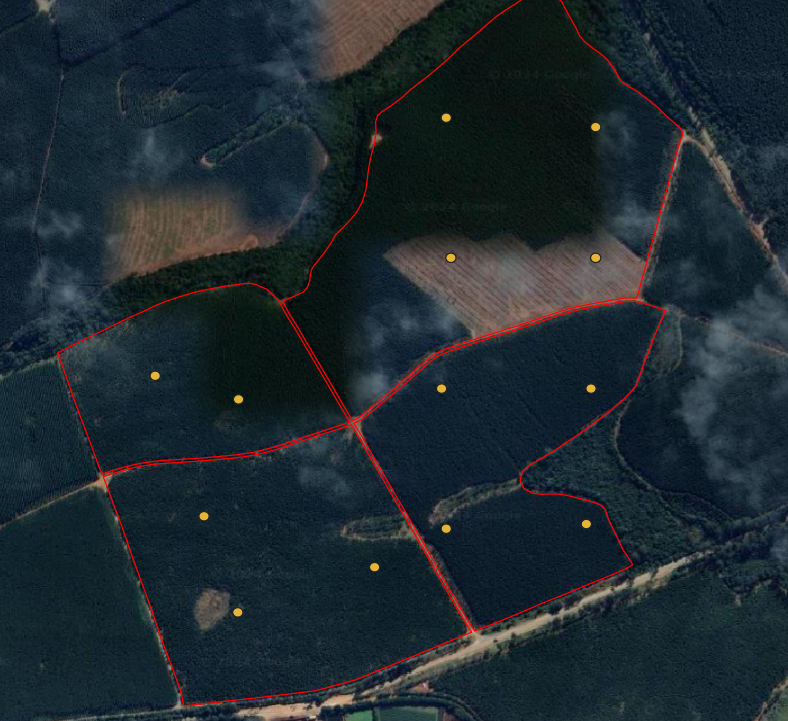
\includegraphics[width=0.4\linewidth]{IMAGES/CAPA} \end{center}

\centerline {Piracicaba, SP – Data de Emissão: 26 de julho de 2024}
\newpage

\tableofcontents

\newpage

\section{Pacotes utilizados no R (colocar breve descrição - já tem uma
descriçãozinha no R passado em
aula)}\label{pacotes-utilizados-no-r-colocar-breve-descriuxe7uxe3o---juxe1-tem-uma-descriuxe7uxe3ozinha-no-r-passado-em-aula}

\subsection{\texorpdfstring{Tidyverse
(\url{https://livro.curso-r.com/4-2-tidyverse.html})}{Tidyverse (https://livro.curso-r.com/4-2-tidyverse.html)}}\label{tidyverse-httpslivro.curso-r.com4-2-tidyverse.html}

O Tidyverse é um pacote guarda-chuva e contém diversas funções úteis
para garantir o dinamismo no script, visualização, processamento e
análise dos dados, modelagem etc.

\begin{figure}

{\centering 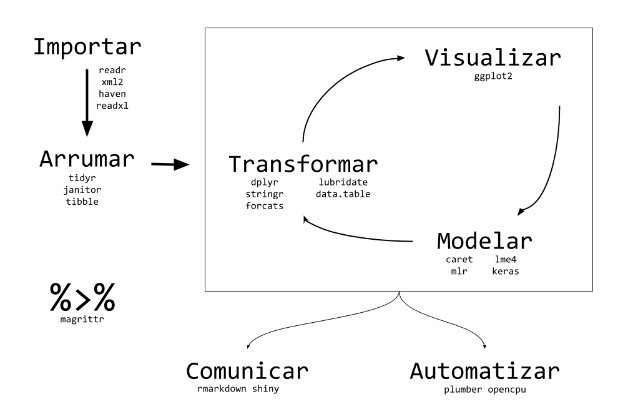
\includegraphics[width=0.6\linewidth]{IMAGES/tidyverse} 

}

\caption{Tidyverse}\label{fig:unnamed-chunk-2}
\end{figure}

\subsection{Sf}\label{sf}

Pacote utilizado para manipulação de objetos do mundo real. Descreve a
forma com que esses objetos podem ser armazenados e importados e quais
operações geométricas podem ser definidas por eles.

\subsection{Tidyterra}\label{tidyterra}

\subsection{Terra}\label{terra}

\subsection{Stars}\label{stars}

\subsection{Tools}\label{tools}

\subsection{RColorBrewer}\label{rcolorbrewer}

\subsection{Progress}\label{progress}

\subsection{Reshape2}\label{reshape2}

\subsection{Mapview}\label{mapview}

\subsection{LidR}\label{lidr}

\subsection{RCSF}\label{rcsf}

\subsection{Future}\label{future}

\newpage

\section{Descrição da área}\label{descriuxe7uxe3o-da-uxe1rea}

A área a ser estudada como ``Fazenda Modelo'' localiza-se no município
de São Miguel Arcanjo (SP), pode ser identificada pelas coordenadas
(-23.86707°, -47.87772°) e possui 129,784 ha, que dividem-se em 4
subtalhões: 301a (18,933 ha), 301d (34,468 ha), 302a (47,602 ha) e 302c
(28,781 ha).

\begin{figure}

{\centering 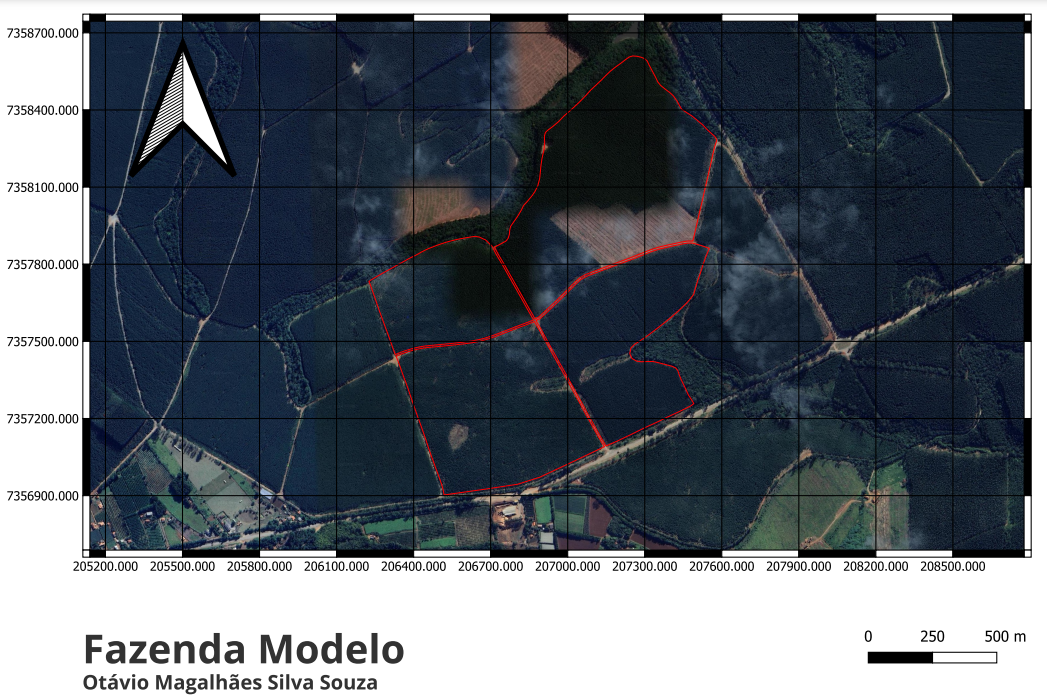
\includegraphics[width=0.6\linewidth]{IMAGES/mapafazendamodelo} 

}

\caption{Mapa da propriedade}\label{fig:unnamed-chunk-3}
\end{figure}
\begin{figure}

{\centering 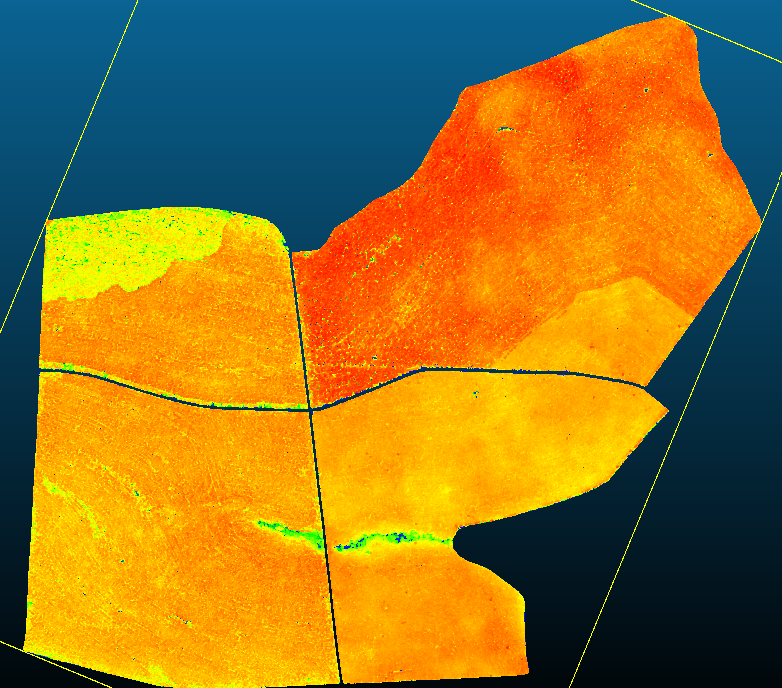
\includegraphics[width=0.4\linewidth]{IMAGES/nuvensnormalizadas} 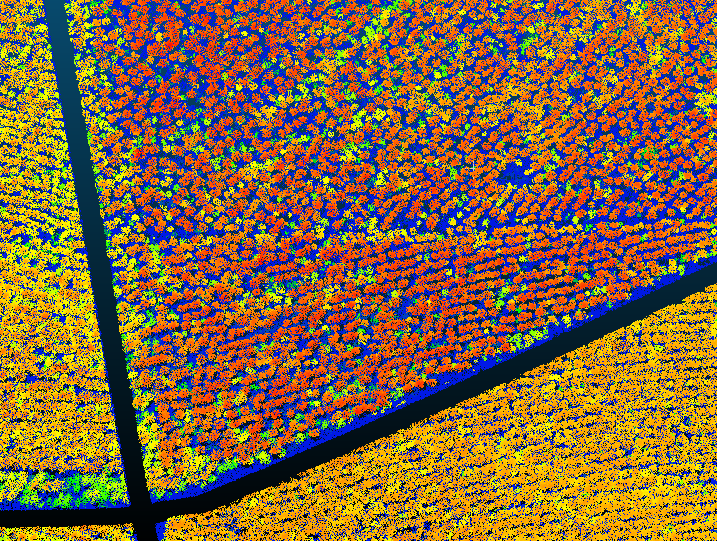
\includegraphics[width=0.4\linewidth]{IMAGES/nuvensnormalizadaszoom} 

}

\caption{Nuvens LiDAR normalizadas}\label{fig:unnamed-chunk-4}
\end{figure}

\newpage

\section{Grid e parcelas já
inventariadas}\label{grid-e-parcelas-juxe1-inventariadas}

A região foi dividida em 3454 parcelas, onde 2960 delas possuem 400m²,
enquanto as outras são menores por estarem na borda e abrangerem áreas
além da área de interesse. Além disso, 13 das parcelas possuem dados de
inventário florestal e podem ser identificadas pelos seguintes Id's:
993, 1526, 1770, 1881, 3165, 3628, 3660, 3730, 5052, 5091, 5106 e 5122.

\begin{figure}

{\centering 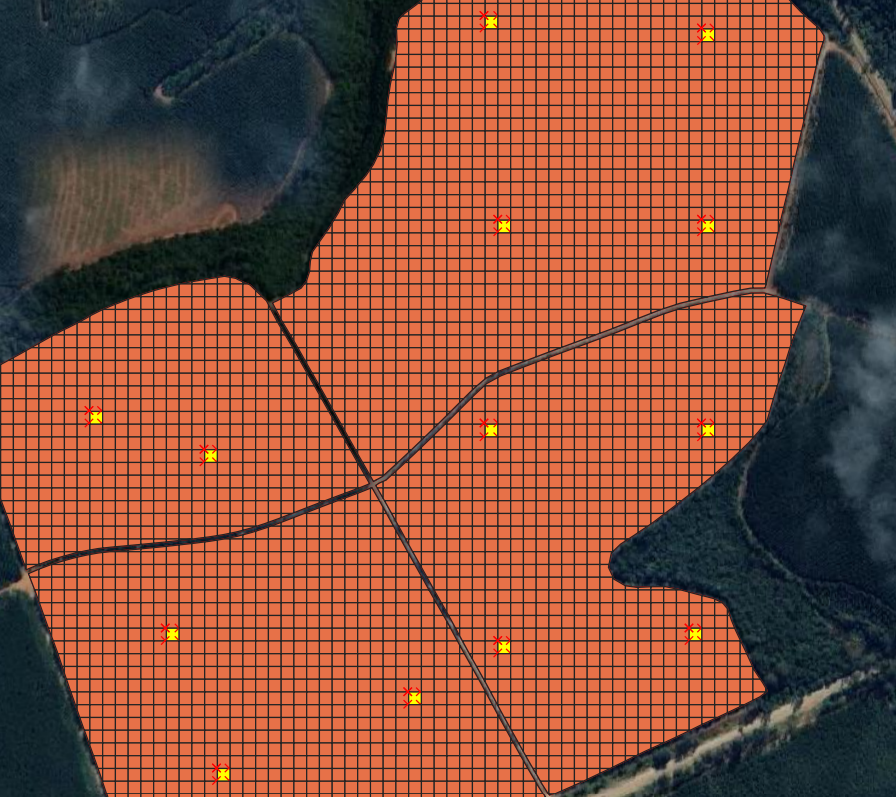
\includegraphics[width=0.4\linewidth]{IMAGES/parcelasinventariadas} 

}

\caption{Parcelas com dados de inventário}\label{fig:unnamed-chunk-5}
\end{figure}
\newpage

\section{Conceitos e definições da Dupla
Amostragem}\label{conceitos-e-definiuxe7uxf5es-da-dupla-amostragem}

A dupla amostragem é composta por duas fases (s1 e s2) - s1: compreende
uma gama de variáveis explanatórias para cada ponto pertencente a s1. As
variáveis explanatórias derivam de informações auxiliares disponíveis em
grande quantidade ao longo da área florestal;\\
- s2: constitui o inventário terrestre feito num número limitado de
subamostras, onde todas pertencem à s1 e fornecem o valor das variáveis
de interesse, ex. densidade local.

Exemplo prático e definições
(\url{https://www.ipef.br/publicacoes/scientia/nr108/cap09.pdf})\\
- O erro amostral (E\%) é calculado a partir do desvio padrão S², que
representa a variação de uma série de médias retiradas da população\\
- A dupla amostragem se divide em duas fases. Na primeira fase há uma
maior intensidade amostral e se é medida a variável auxiliar, que deve
ser de mensuração facilitada. Na segunda fase a intensidade amostral é
menor e se mede a variável de interesse e a variável auxiliar, pois será
calculado um estimador de regressão entre as duas. (existe uma diferença
entre estimadores de regressão e de razão - estudar)\\
- A alta correlação entre métricas LiDAR e parâmetros biofísicos da
floresta justificam a adoção da tecnologia na primeira fase da DA, além
de reduzir a intensidade amostra (custo e trabalho) - Primeira fase:
lançamento das parcelas e sobrevôo com o LiDAR\\
- Etapas (2a fase): mensuração de variáveis das árvores (ex. DAP),
medição de algumas árvores para gerar modelo hipsométrico, que será
usado para descobrir a altura das outras árvores, cálculo do volume
também por modelo e extrapolação do volume da parcela.\\
- O estimador de regressão (estudar) do VTCC deve relacionar a(s)
variável(eis) auxiliar(es) e também compreende a outros índices
(constantes para cada região)\\
- O desvio padrão, intervalo de confiança etc são feitos depois

\begin{figure}

{\centering 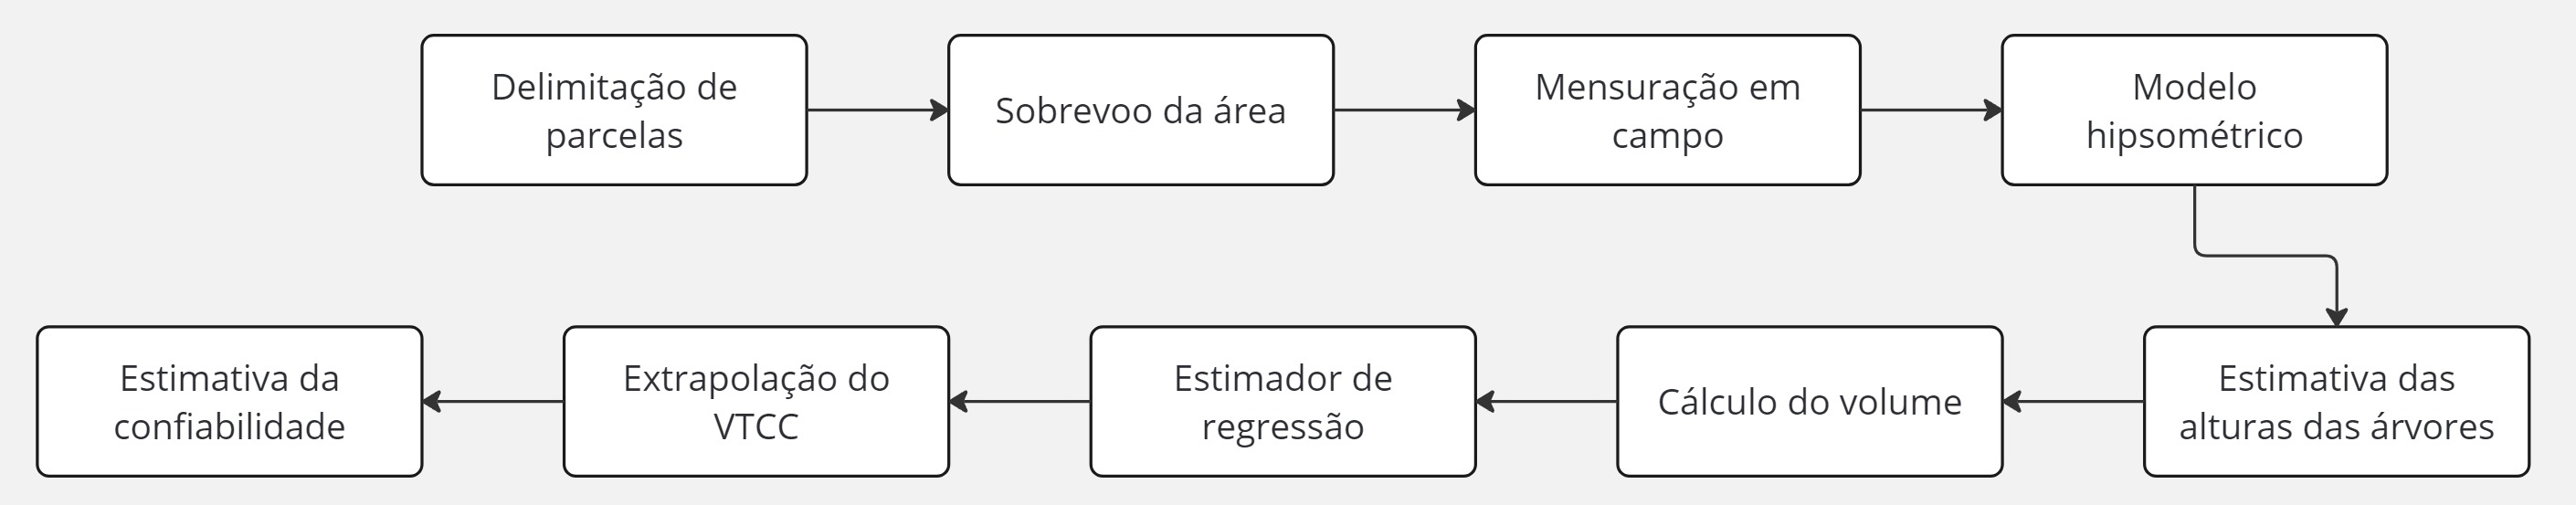
\includegraphics[width=0.45\linewidth]{IMAGES/fluxograma-da-lidar-e-campo} 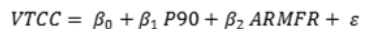
\includegraphics[width=0.45\linewidth]{IMAGES/eq-estimador-regressao} 

}

\caption{Fluxograma DA e estimador de regressão para VTCC}\label{fig:unnamed-chunk-6}
\end{figure}

\section{Fluxograma e etapas Dupla
amostragem}\label{fluxograma-e-etapas-dupla-amostragem}

\begin{figure}

{\centering 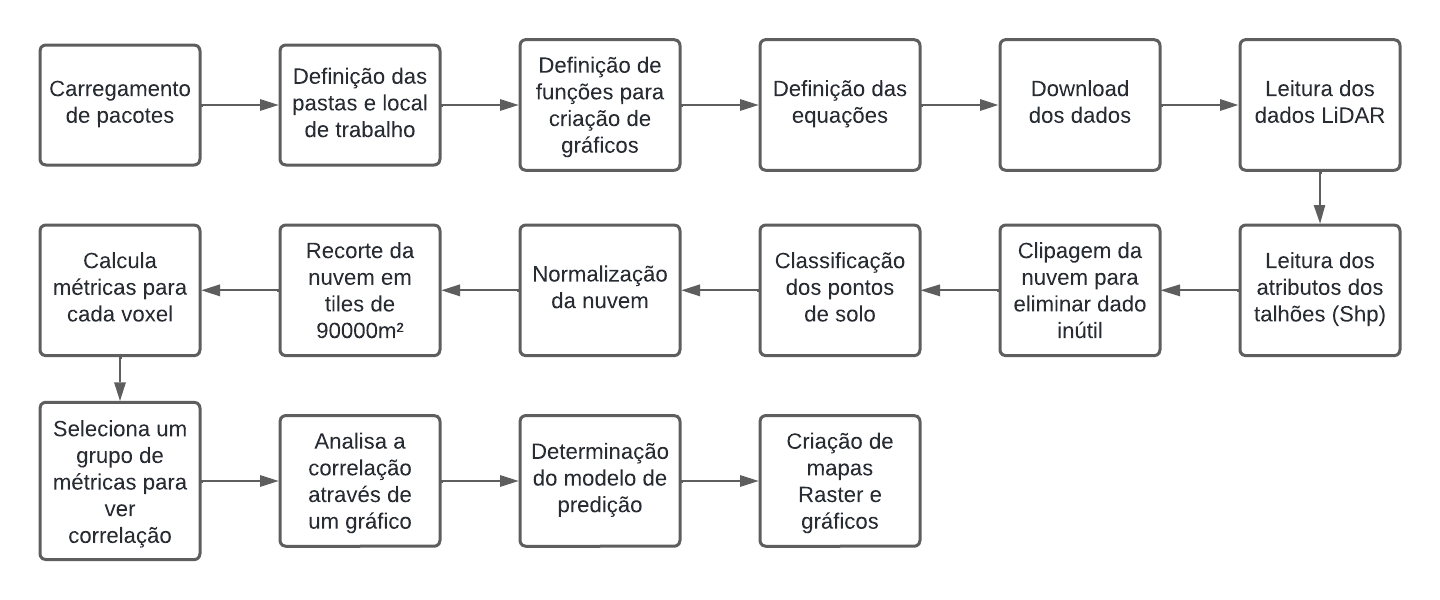
\includegraphics[width=0.8\linewidth]{IMAGES/fluxogramaDA} 

}

\caption{Fluxograma das etapas de processamento de dados LiDAR para fins de inventário florestal}\label{fig:unnamed-chunk-7}
\end{figure}

\begin{enumerate}
\def\labelenumi{\arabic{enumi}.}
\tightlist
\item
  Carregamento dos pacotes
\end{enumerate}

\begin{enumerate}
\def\labelenumi{\roman{enumi}.}
\tightlist
\item
  Diversos são os pacotes carregados. Os nomes e a utilidade de cada um
  estão descritos na primeira seção do documento. \newpage
\end{enumerate}

\begin{enumerate}
\def\labelenumi{\arabic{enumi}.}
\setcounter{enumi}{1}
\tightlist
\item
  Definição das pastas e local de trabalho
\end{enumerate}

\begin{itemize}
\tightlist
\item
  GitHub

  \begin{enumerate}
  \def\labelenumi{\roman{enumi}.}
  \tightlist
  \item
    C: - pasta raiz
  \item
    GitRepo - diretório em que estão agrupados os arquivos a serem
    upados no GitHub
  \item
    PRJ\_FAZENDAMODELO - pasta do projeto
  \item
    RMD - código e arquivos utilizados na redação do presente documento
  \item
    RESULTADOS - plot da matriz de correlação
  \item
    BATCHR - arquivo tipo R com os scripts utilizados no pré e
    pós-processamento dos dados
  \item
    SAIDASSIG - arquivos gerados no QGIS
  \item
    SHAPES - arquivos de entrada para uso no SIG
  \end{enumerate}
\item
  LiDAR

  \begin{enumerate}
  \def\labelenumi{\roman{enumi}.}
  \tightlist
  \item
    C: - pasta raiz
  \item
    LiDAR - agrupa todos as nuvens de pontos utilizadas no script
  \item
    PRJ\_FAZENDAMODELO - pasta do projeto
  \item
    NUVENS - onde se localizam as nuvens de pontos
  \item
    A13 - reúne as nuvens do ano de 2013
  \item
    TALHOES - nuvem segregada por talhão
  \item
    NoNORM - nuvens com solo classificado
  \item
    SiNORM - nuvens com solo classificado e normalizadas
  \item
    RSTR\_qua - raster apresentando a estimativa da variável de
    interesse para cada talhão
  \end{enumerate}
\end{itemize}

\begin{figure}

{\centering 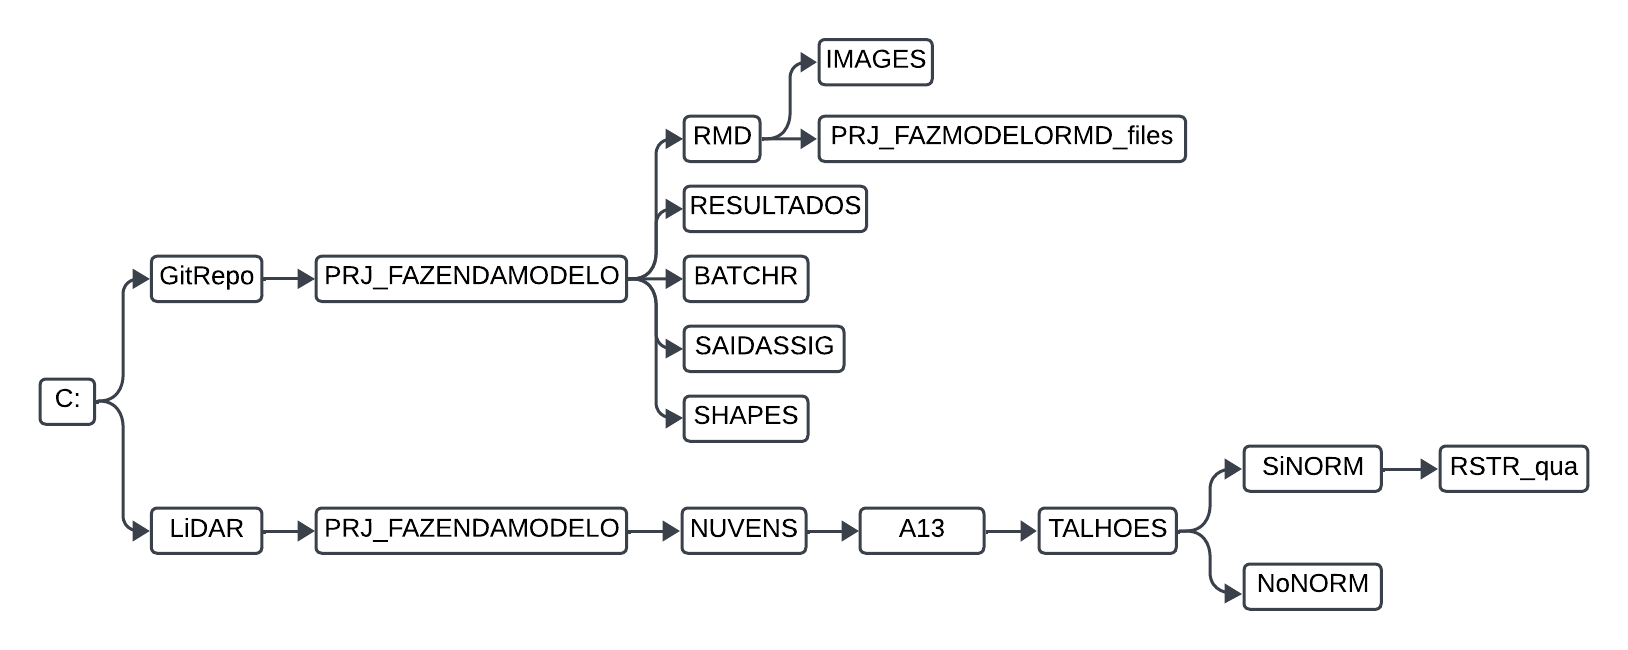
\includegraphics[width=0.8\linewidth]{IMAGES/organizacao-pastas} 

}

\caption{Organização dos diretórios}\label{fig:unnamed-chunk-8}
\end{figure}

\newpage

\begin{enumerate}
\def\labelenumi{\arabic{enumi}.}
\setcounter{enumi}{2}
\tightlist
\item
  Definição das funções para criação dos gráficos
\end{enumerate}

\newpage

\begin{enumerate}
\def\labelenumi{\arabic{enumi}.}
\setcounter{enumi}{3}
\tightlist
\item
  Definição das equações (estudar quais são)
\end{enumerate}

\newpage

\begin{enumerate}
\def\labelenumi{\arabic{enumi}.}
\setcounter{enumi}{4}
\tightlist
\item
  Download e leitura dos dados LiDAR
\end{enumerate}

\begin{enumerate}
\def\labelenumi{\roman{enumi}.}
\tightlist
\item
  Ao todo foram baixadas 6 nuvens de pontos LiDAR, que antes do
  processamento encontravam-se da seguinte maneira:
\end{enumerate}

\begin{figure}

{\centering 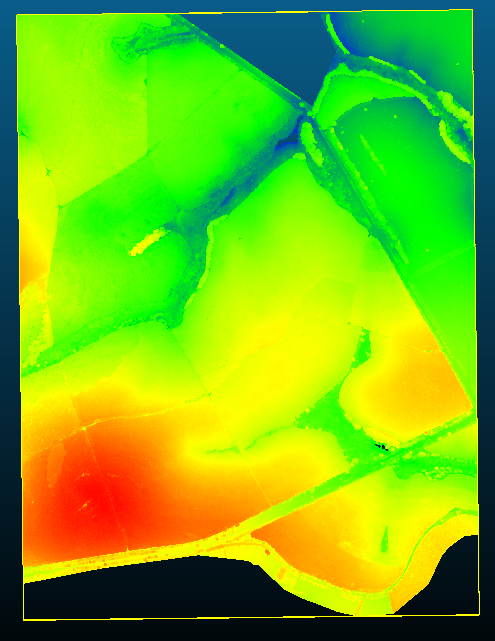
\includegraphics[width=0.4\linewidth]{IMAGES/pre-clipagem-passo8} 

}

\caption{Nuvens de pontos LiDAR pré-processadas}\label{fig:unnamed-chunk-9}
\end{figure}

\begin{enumerate}
\def\labelenumi{\roman{enumi}.}
\setcounter{enumi}{1}
\tightlist
\item
  As nuvens foram baixadas pelo seguinte link:
  \url{https://github.com/FlorestaR/dados/blob/main/5_LIDARF/Modelo/CLOUDS/}
\end{enumerate}

\newpage
6

. Download e leitura dos dados em Shapefile\\
i. Os shapes foram baixados pelo seguinte link:
\url{https://github.com/FlorestaR/dados/blob/main/5_LIDARF/Modelo/SHAPES}

\begin{figure}

{\centering 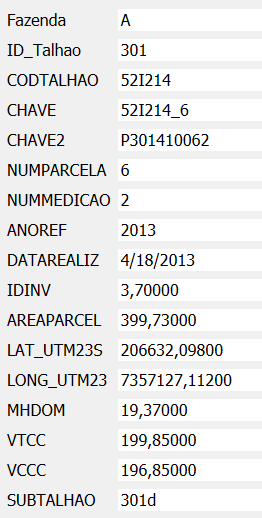
\includegraphics[width=0.5\linewidth]{IMAGES/atributosinventariadas} 

}

\caption{Dados contidos nas parcelas inventariadas}\label{fig:unnamed-chunk-10}
\end{figure}

\newpage
7

. Clipagem da nuvem para eliminação de dados indesejados (mostrar nuvem
antes e depois)\\
Antes da clipagem: 68mi pontos\\
Após clipagem: 18mi pontos

\begin{figure}

{\centering 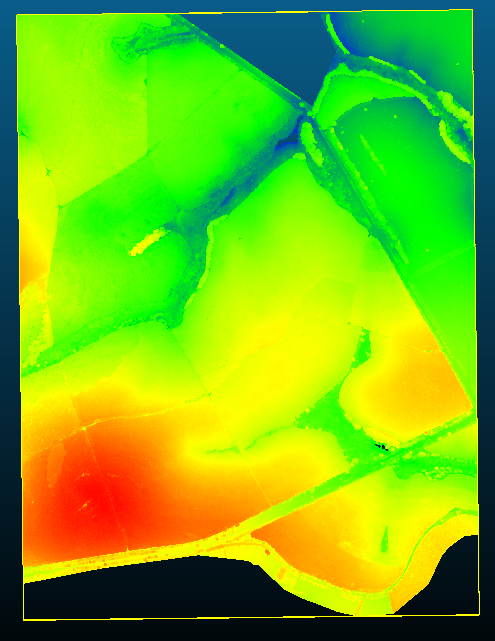
\includegraphics[width=0.4\linewidth]{IMAGES/pre-clipagem-passo8} 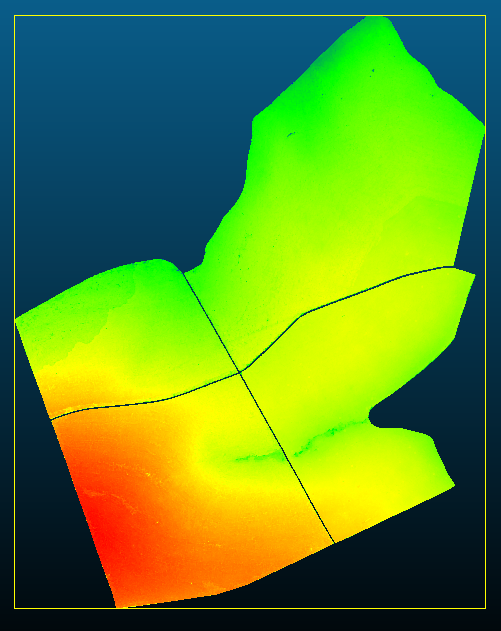
\includegraphics[width=0.4\linewidth]{IMAGES/pos-clipagem-passo8} 

}

\caption{Comparativo entre as nuvens de pontos antes e após a clipagem}\label{fig:unnamed-chunk-11}
\end{figure}

\newpage
8

. Classificação

\begin{figure}

{\centering 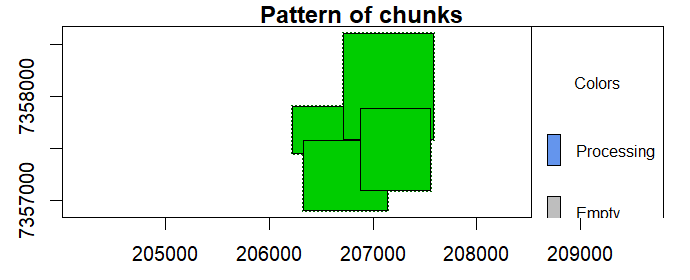
\includegraphics[width=0.4\linewidth]{IMAGES/classificacao-pontos-de-solo} 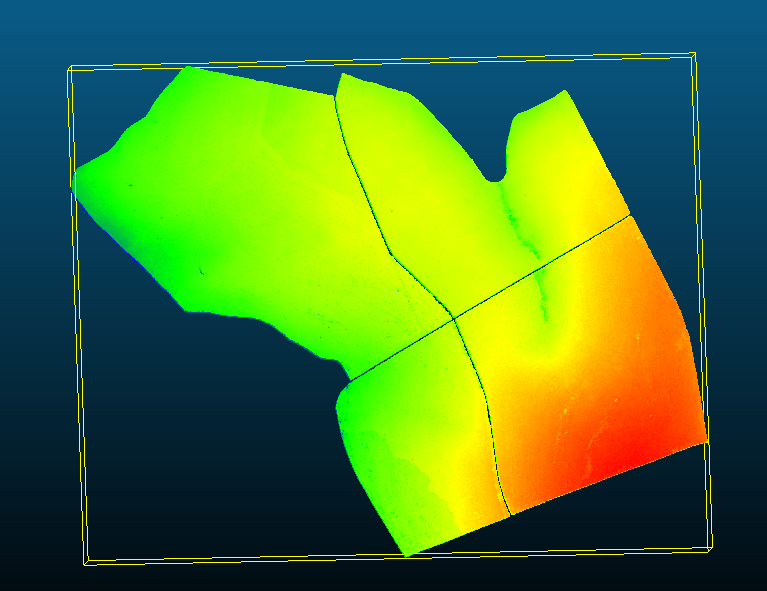
\includegraphics[width=0.4\linewidth]{IMAGES/nuvem-com-pontos-de-solo-classificados-mas-sem-normalizacao} 

}

\caption{Processamento e resultado da classificação de solo das nuvens LiDAR}\label{fig:unnamed-chunk-12}
\end{figure}
\newpage
9

. Normalização i. A etapa de normalização tem por finalidade nivelar
toda a nuvem e é um passo que está diretamente correlacionado à
classificação do solo.

\begin{figure}

{\centering 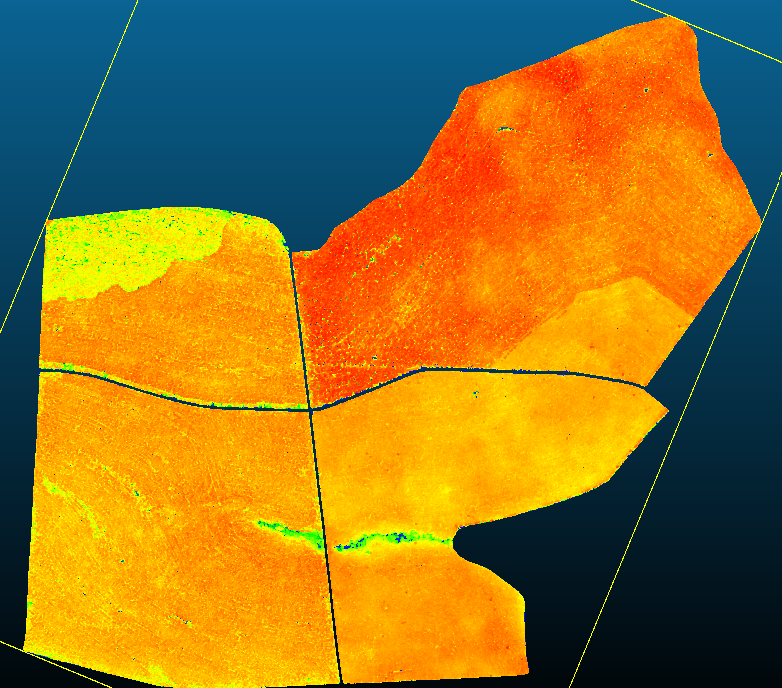
\includegraphics[width=0.4\linewidth]{IMAGES/nuvensnormalizadas} 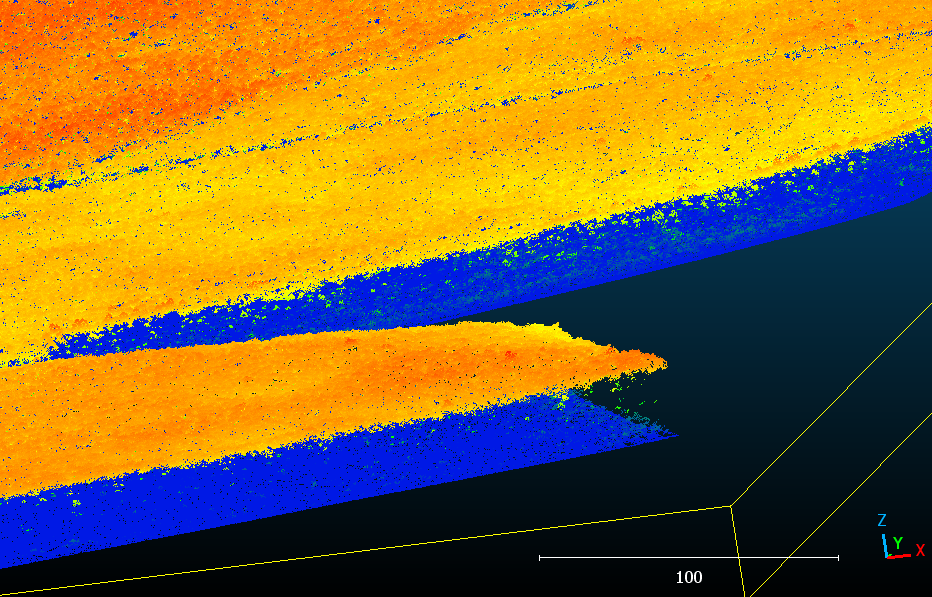
\includegraphics[width=0.4\linewidth]{IMAGES/nivelamento} 

}

\caption{Resultado da normalização das nuvens}\label{fig:unnamed-chunk-13}
\end{figure}
\newpage
10

. Recorte da nuvem em tiles 300x300m O recorte da nuvem em tiles menores
tme a função de facilitar o processamento dos dados, tornando-o mais
rápido e dinâmico

\begin{figure}

{\centering 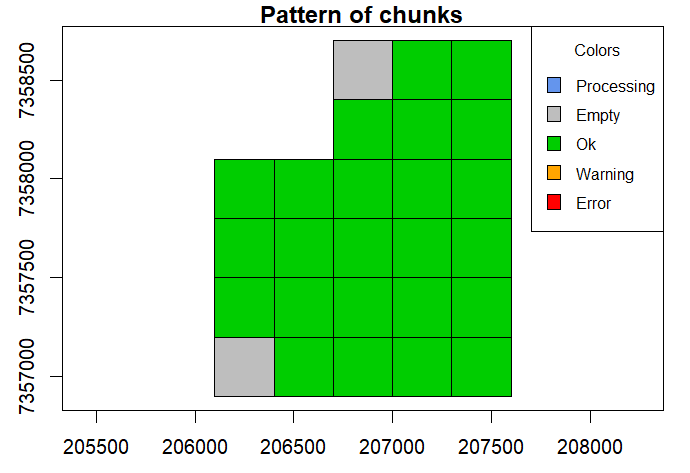
\includegraphics[width=0.5\linewidth]{IMAGES/Retile} 

}

\caption{Retile da nuvem em quadrados de 300x300m}\label{fig:unnamed-chunk-14}
\end{figure}
\newpage

\begin{enumerate}
\def\labelenumi{\arabic{enumi}.}
\setcounter{enumi}{10}
\tightlist
\item
  Cálculo de métricas para cada voxel (explicar voxel)
\end{enumerate}

\begin{figure}

{\centering 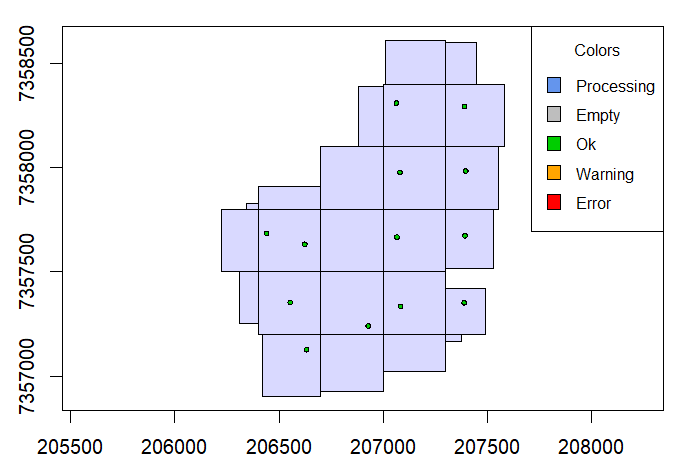
\includegraphics[width=0.5\linewidth]{IMAGES/calculo-metricas-voxel} 

}

\caption{Cálculo das métricas para cada voxel}\label{fig:unnamed-chunk-15}
\end{figure}
\newpage
12

. Seleção de um grupo de métricas para estudo de correlação

\begin{figure}

{\centering 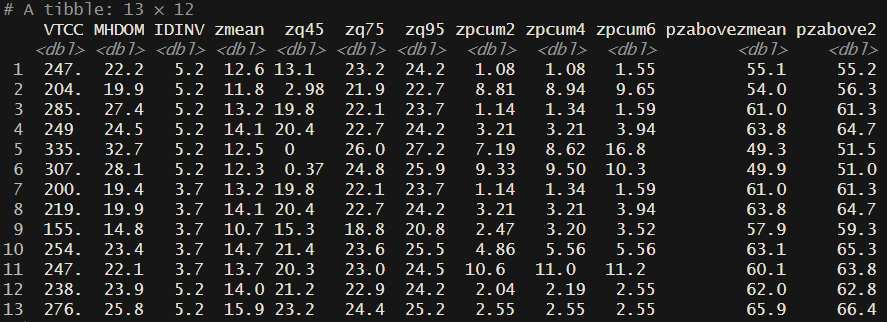
\includegraphics[width=0.5\linewidth]{IMAGES/tb-subgrupo-de-metricas-p-analise} 

}

\caption{Tabela com as métricas escolhidas}\label{fig:unnamed-chunk-16}
\end{figure}
\newpage
13

. Análise da correlação por meio de gráfico (falar do gráfico)

\begin{figure}

{\centering 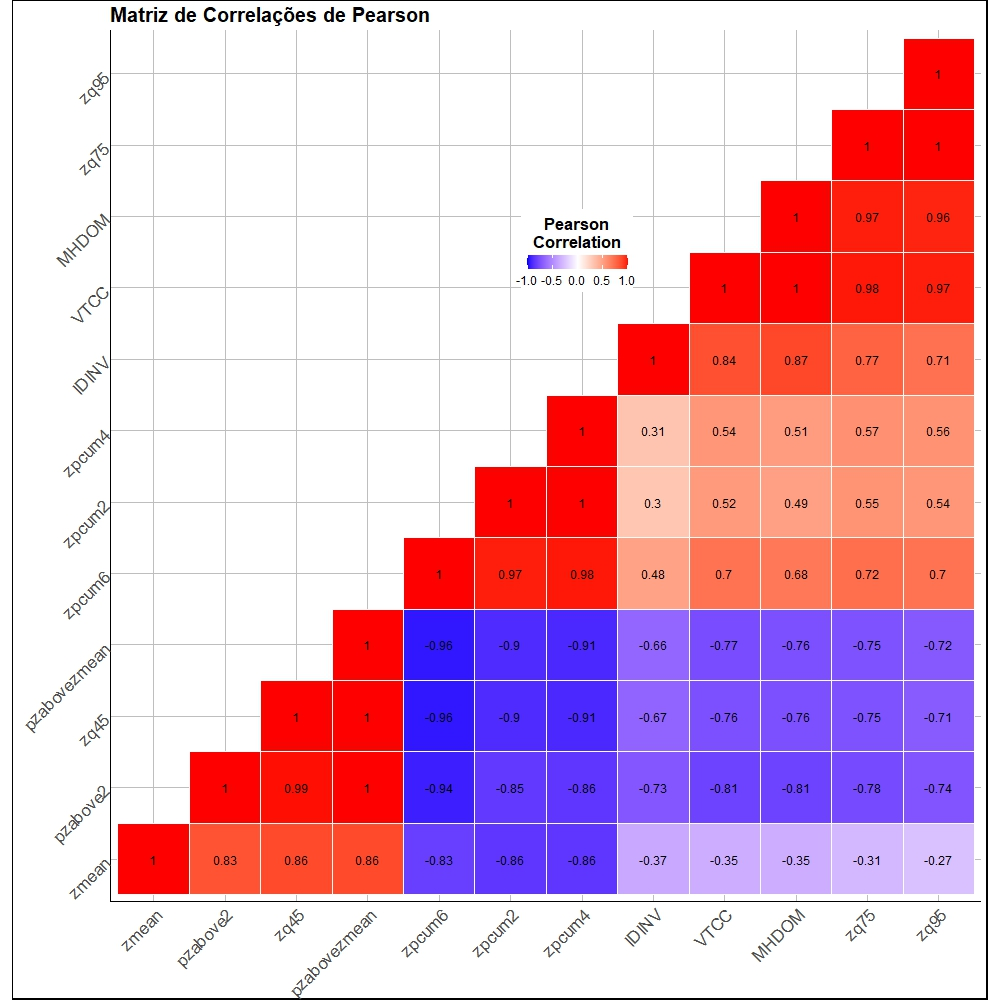
\includegraphics[width=0.5\linewidth]{IMAGES/MatrizDeCorrelacoes} 

}

\caption{Resultado da análise de correlação}\label{fig:unnamed-chunk-17}
\end{figure}
\newpage
14

. Determinação do modelo de predição

\begin{figure}

{\centering 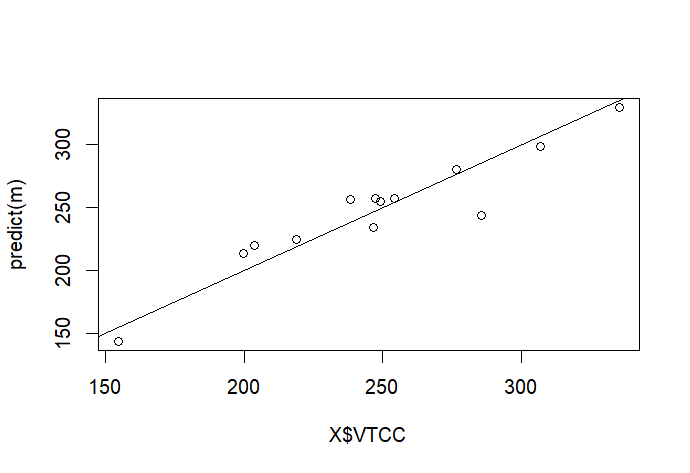
\includegraphics[width=0.5\linewidth]{IMAGES/analise-de-regressao} 

}

\caption{nao sei}\label{fig:unnamed-chunk-18}
\end{figure}
\newpage
15

. Criação de mapas raster e gráficos \newpage

\section{Fluxograma e etapas Tripla
amostragem}\label{fluxograma-e-etapas-tripla-amostragem}

Composta por 3 fases, s0, s1 e s2:\\
- O princípio básico é o de que as variáveis explanatórias derivadas das
informações auxiliares estão disponíveis em duas frequências diferentes.
A fase s0 fornece informações sobre toda a área, enquanto s1 possui
dados adicionais de amostras de s0. Logo, a partir da informação
terrestre coletada de um número x de parcelas de campo (1 camada de
informação) é possível aferir sobre informações adicionais para outras
parcelas a partir do uso de preditores (2 camadas de informação) e, por
fim, o LiDAR coleta dados sobre todas as parcelas (3 camadas de
informação).\\
- Logo, a motivação por trás da TA é a de que a gama de informações de
s1 adiciona alto poder preditivo às variáveis disponíveis para todas as
parcelas da área (s0)

\begin{figure}

{\centering 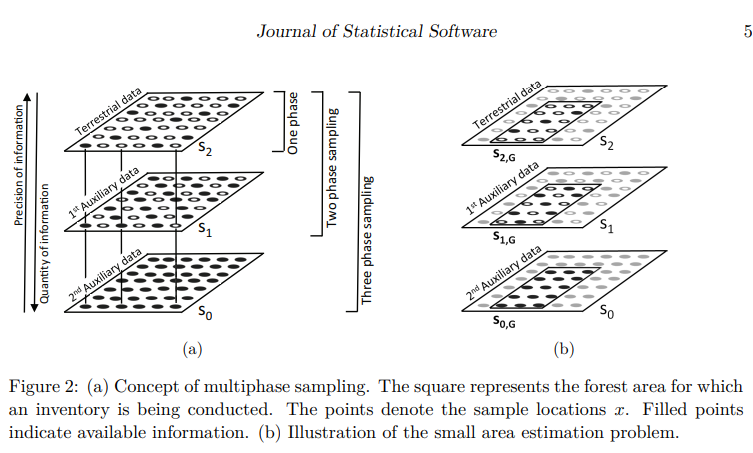
\includegraphics[width=0.5\linewidth]{IMAGES/esquematizacao-TA} 

}

\caption{Esquema TA com Lidar}\label{fig:unnamed-chunk-19}
\end{figure}

Estimativas de pequenas áreas (small area estimation)\\
- Para sub áreas da floresta onde há pouca informação terrestre, como em
G na figura acima. Para essas áreas, o uso da amostragem multifásica
pode ser mais eficiente, já que utilizam um número reduzido de parcelas
em campo para chegar à mesma precisão da ACE e ACS. Por outro lado, a
sub área em questão pode ser pequena demais para justificar a adoção de
um modelo de regressão separado, uma vez que este pode resultar em um
intervalo de confiança indesejadamente abrangente;\\
- A ideia, então, é a de utilizar toda a riqueza de informações presente
nas amostras de S2 para ajustar o modelo (equação utilizada para o
cálculo de uma variável de interesse) e aplicá-lo para a sub área em
questão.\\
- O potencial viés que surge da aplicação do modelo na sub área é
corrigido pelo uso de modelos residuais empíricos derivados da área
amostrada em campo. (não entendi direito essa parte) - trecho no texto:
The potential bias of applying that model in G is then corrected for by
using the empirical model residuals derived from that small area.\\
- Caso não existam parcelas de campo na sub área, então deve-se aceitar
o viés na estimativa e no modelo. São essas as estimativas sintéticas,
mas apesar do viés é possível calcular a sua variação.

DESIGN-BASED VS MODEL-DEPENDENT APPROACH (ver dps)\\
- Model-dependent approach: as parcelas amostrais são fixas e as
observações retiradas desses locais são assumidas como variáveis
aleatórias, assim como a floresta assume o papel de ser o meio
realizador desse processo estocástico (?????? o que isso significa?).
Embora os locais das parcelas possam ser arbitrariamente escolhidos, o
modelo deve escrever adequadamente o processo estocástico, a fim de
garantir resultados parciais. (????)\\
- Os estimadores do forestinventory se baseiam na design-based approach.
Design-based approach baseia-se na randomização dos locais de amostra de
forma uniforme e independente. Logo, a floresta por si só e qualquer
valor de densidade local de x (pertencente a) F (floresta) são fixos e
não um resultado de um processo estocástico (estudar). (???)\\
- Na estrutura do Model-dependent approach as parcelas são fixas e
resultam em um processo estocástico GPT: what is the difference between
design-based approach and model-dependent approach?

\end{document}
